\documentclass{beamer}
\usepackage[utf8]{inputenc}
\usepackage[]{amsmath}
\usepackage{graphicx}
\usepackage{physics}
\usepackage{subcaption} % package pour faire des subfigures
\usepackage{multirow} % package pour multirow/multicolumn
\usepackage{booktabs} % package pour top/mid/bottom rule
\usepackage{tcolorbox} % toujours plus de boites
\usepackage[backend=biber]{biblatex}


\addbibresource{Biblio_dbl_quantum.bib}

%\bibliographystyle{stylename}
%\bibliography{Biblio_dbl_quantum}

\title{Dipolar interactions in dense ensembles of Nitrogen-Vacancy centers}
\author{Clément Pellet-Mary, Maxime Perdriat, Gabriel Hétet}
\date{Nano-optics group}

\mode<presentation> {\usetheme{Rochester}}

\begin{document}
\begin{frame}
\maketitle
\begin{center}
\includegraphics[width=\textwidth,height=0.3\textheight,keepaspectratio]{logos}
\end{center}
\end{frame}
%\begin{frame}{Outline}
%\tableofcontents
%\end{frame}
%\section{Physics of the NV center}
\begin{frame}{What are NV centers?}
\centering
\includegraphics[width=\textwidth,height=0.9\textheight,keepaspectratio]{Slide  NV properties}
\end{frame}


\begin{frame}{What are NV centers good at ?}
\begin{itemize}
\item Good optical properties : quantum yield $> 0.9$, photostable
%\pause
\medskip
\item Good spin properties : $T_1\approx\ \rm ms$ and $T_2^*\sim \mu$s at 300 K.
%\pause
\medskip
\item Optical polarization (up to 90\%) and readout (fidelity up to 0.3) of the spin at room temperature
\end{itemize}
%\pause
\bigskip
$\to$ One of the most versatile spin qubit at room temperature
\end{frame}

\begin{frame}{What are NV centers being used for ?}
$\bullet$ Quantum memories :
\begin{center}
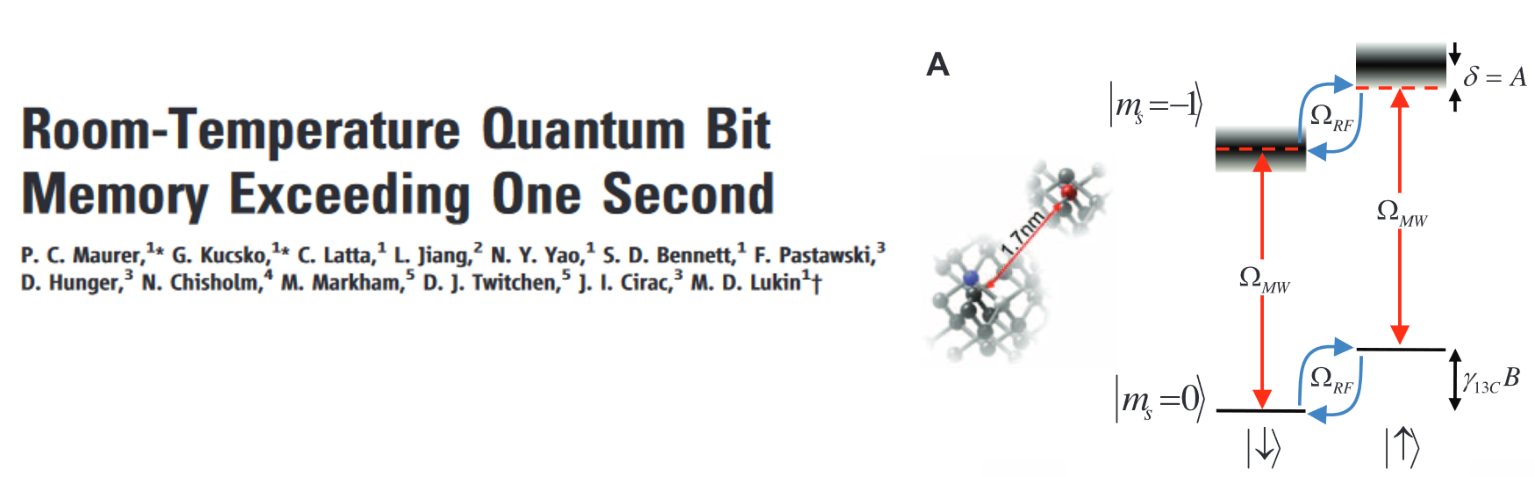
\includegraphics[width=0.8\textwidth,height=0.9\textheight,keepaspectratio]{mémoire}
\end{center}
%\pause

$\bullet$ Intrication :
\begin{center}
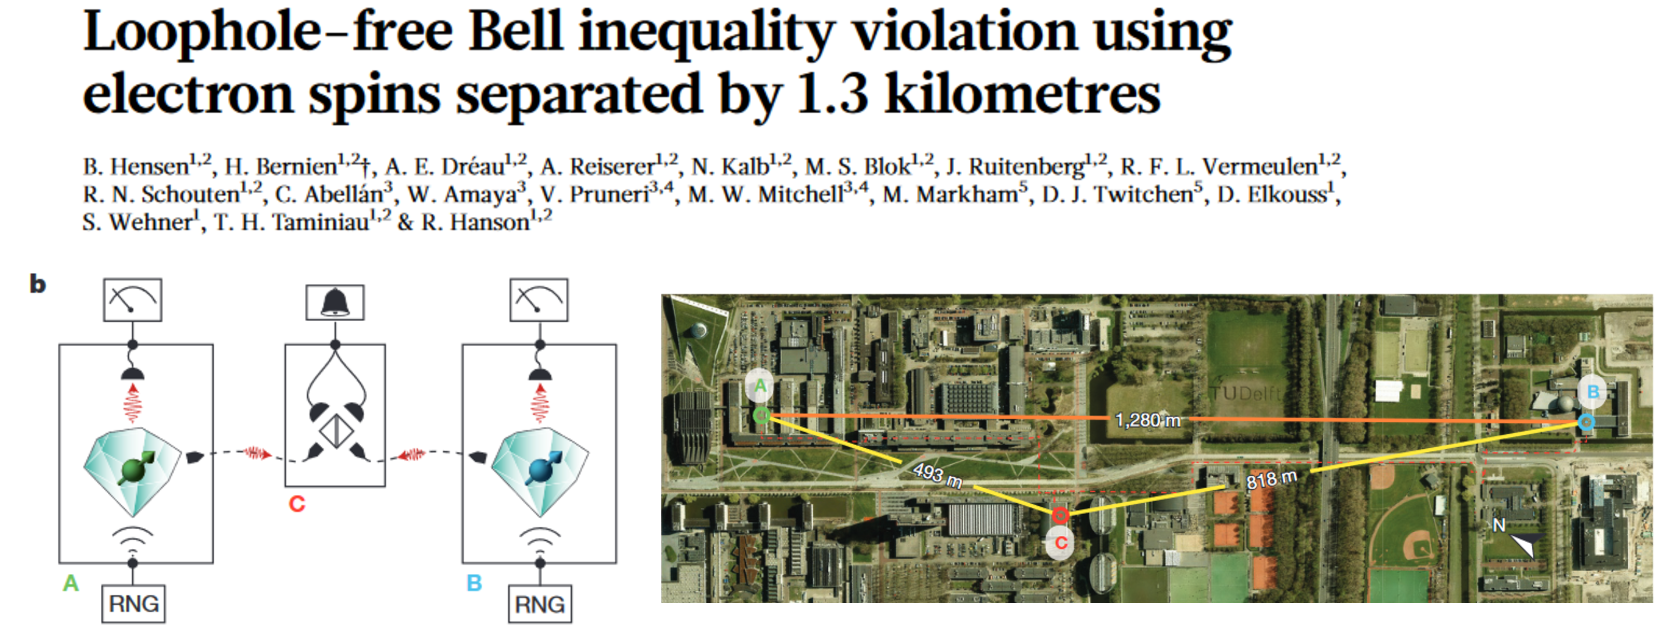
\includegraphics[width=0.8\textwidth,height=0.9\textheight,keepaspectratio]{Intrication}
\end{center}
\end{frame}

\begin{frame}{Magnetomtry with NV centers : big or small}
$\bullet$ AFM nano-scale magnetomtry :
\begin{center}
\includegraphics[width=0.65\textwidth,height=0.9\textheight,keepaspectratio]{magneto AFM}
\end{center}

%\pause

$\bullet$ Diamond magnetic microscopy :
\begin{center}
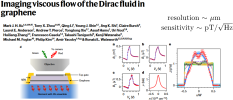
\includegraphics[width=0.65\textwidth,height=0.9\textheight,keepaspectratio]{magneto graphene}
\end{center}
\end{frame}

\begin{frame}{Context of my PhD work : new physics with dense ensemble of NV centers}
\begin{itemize}
\item To increase the magnetic field sensitivity we need to increase the density of NV centers
%\pause
\item Chemists and material scientists have made huge progress to grow NV-rich diamond with little other impurities 
\begin{center}
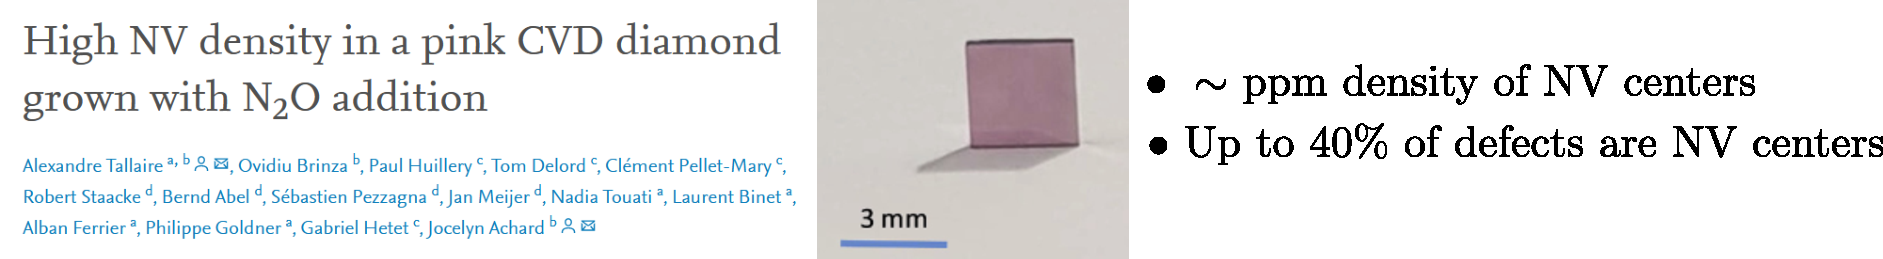
\includegraphics[width=\textwidth,height=0.2\textheight,keepaspectratio]{diamant Alex}
\end{center}
%\pause
\item When the defects density reaches a critical point, many body effects start to appear due to dipole-dipole interaction and charge transfer (3 ppm of NV = 30 kHz dipole coupling rate between NV neighbors)
\end{itemize}
\end{frame}
\begin{frame}{Basic example : Optically Detected Magnetic Resonance (ODMR)}
\centering
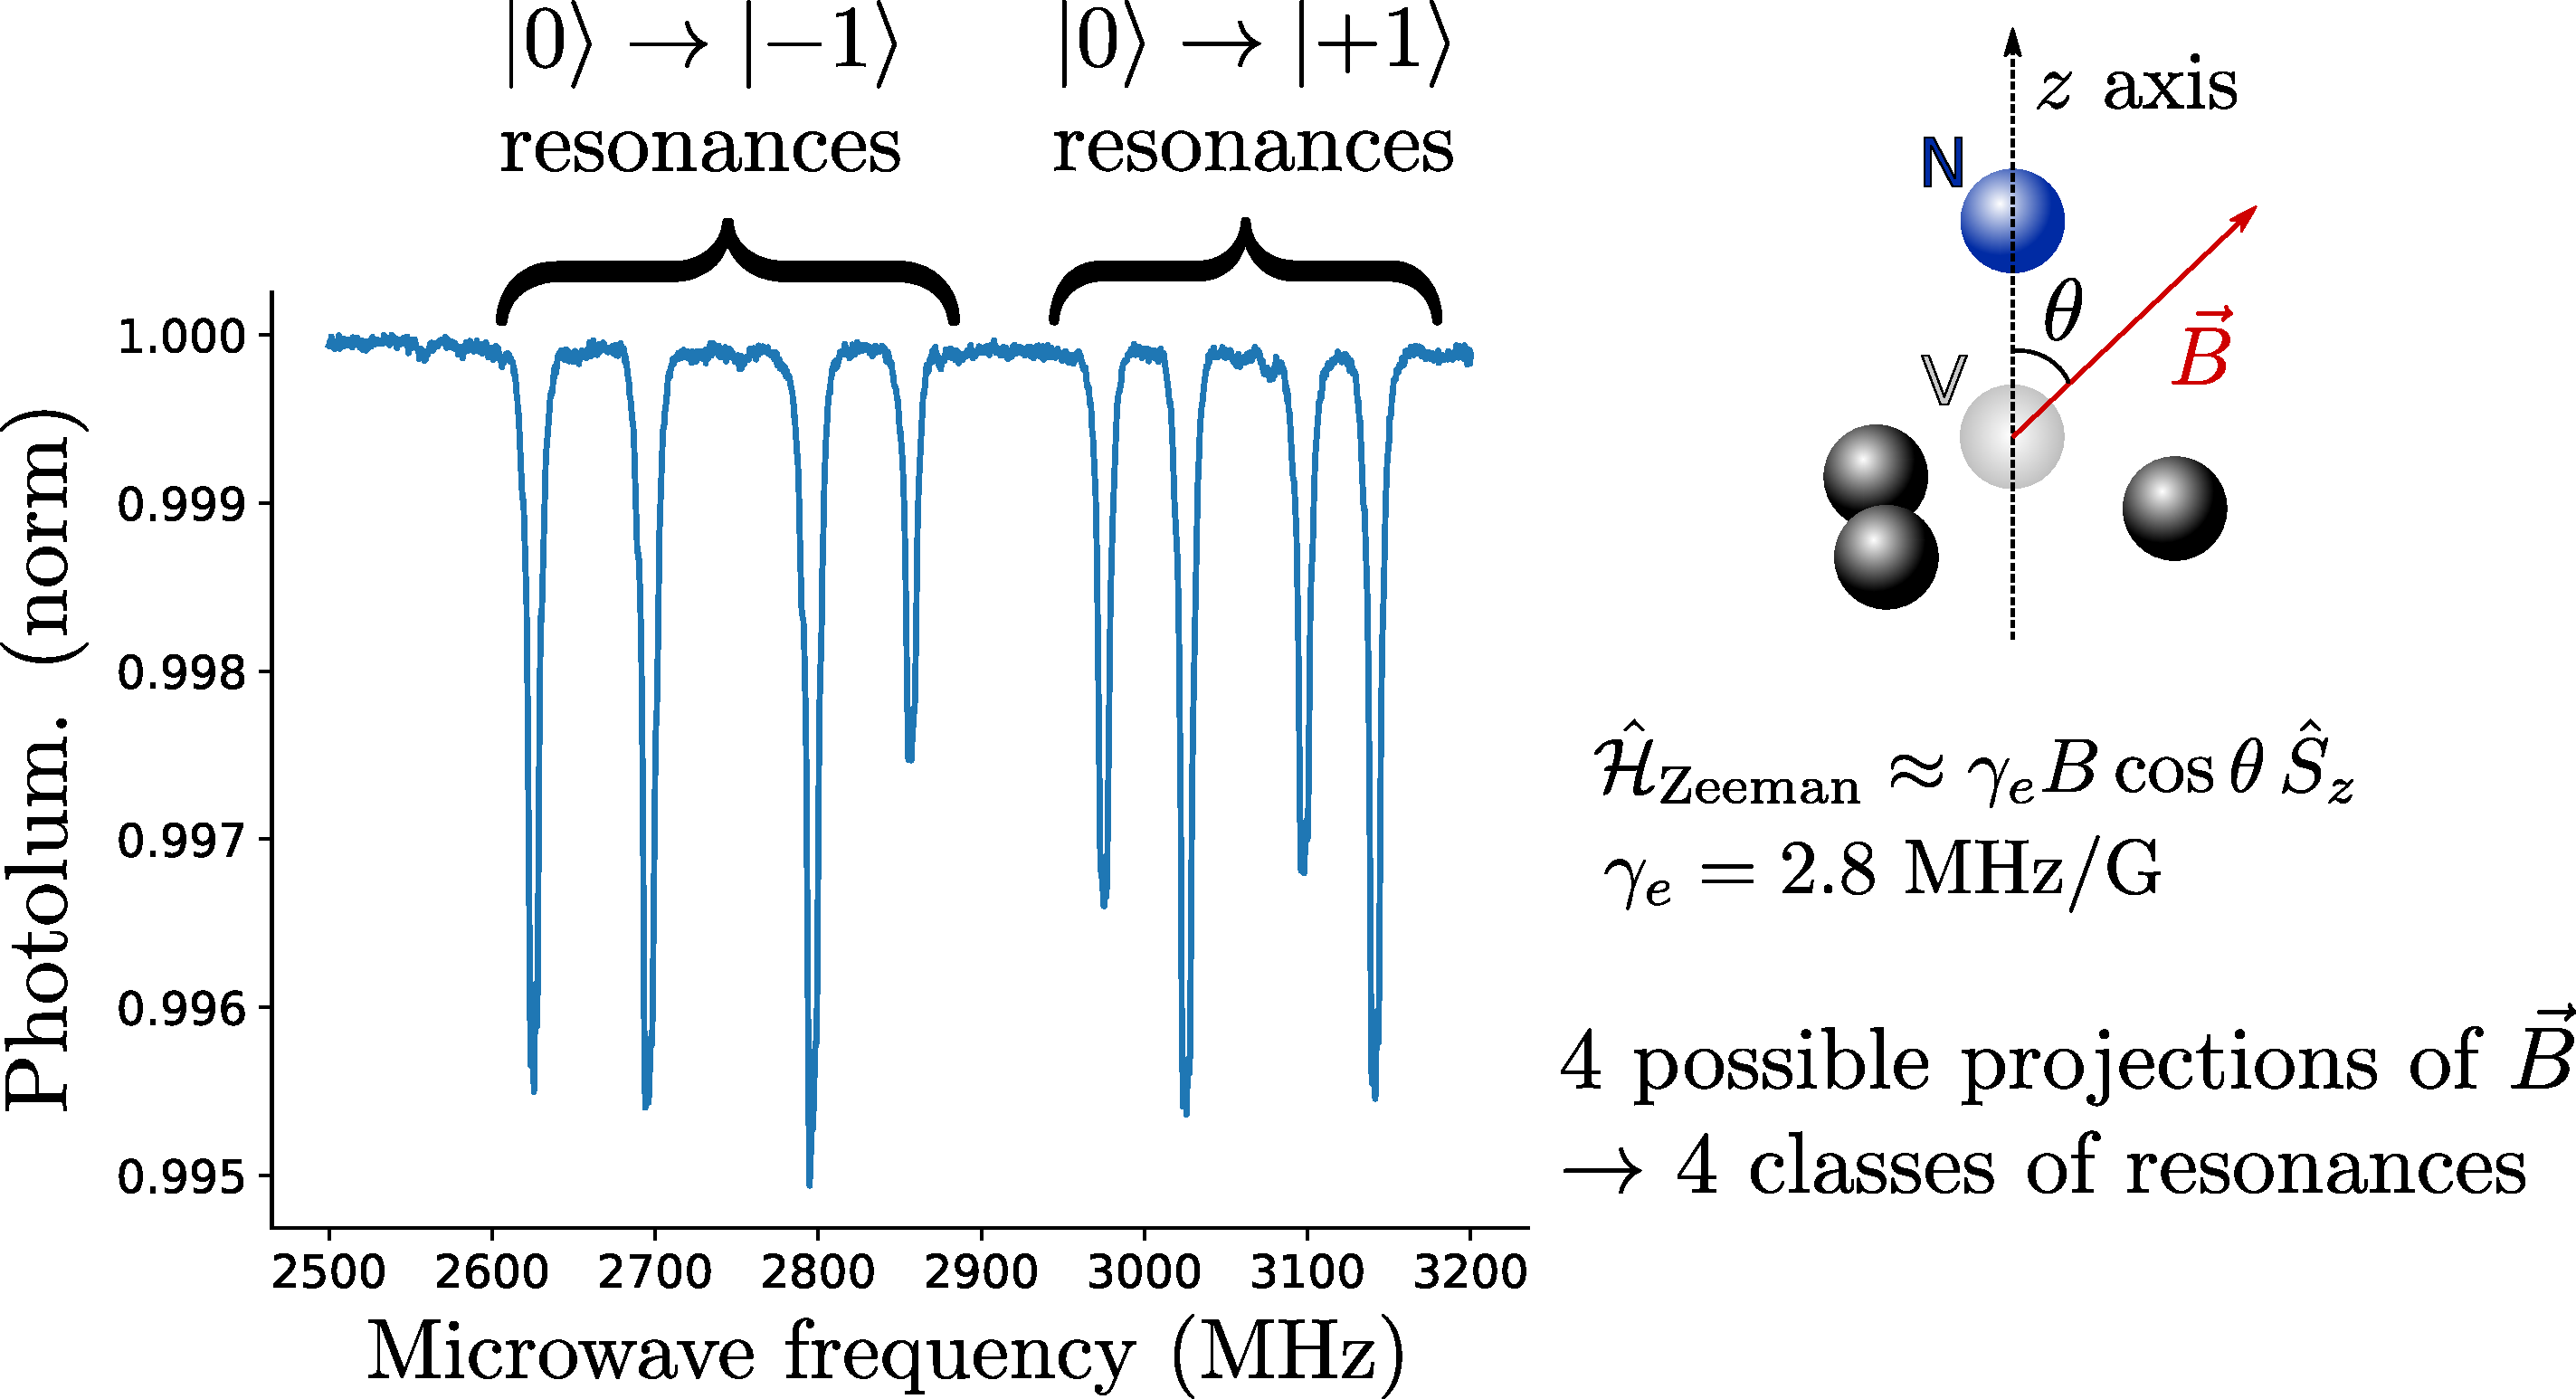
\includegraphics[width=\textwidth,height=0.9\textheight,keepaspectratio]{slide ODMR}
\end{frame}

\begin{frame}{Modification of the spin $T_1$ due to resonant dipole coupling}
\centering
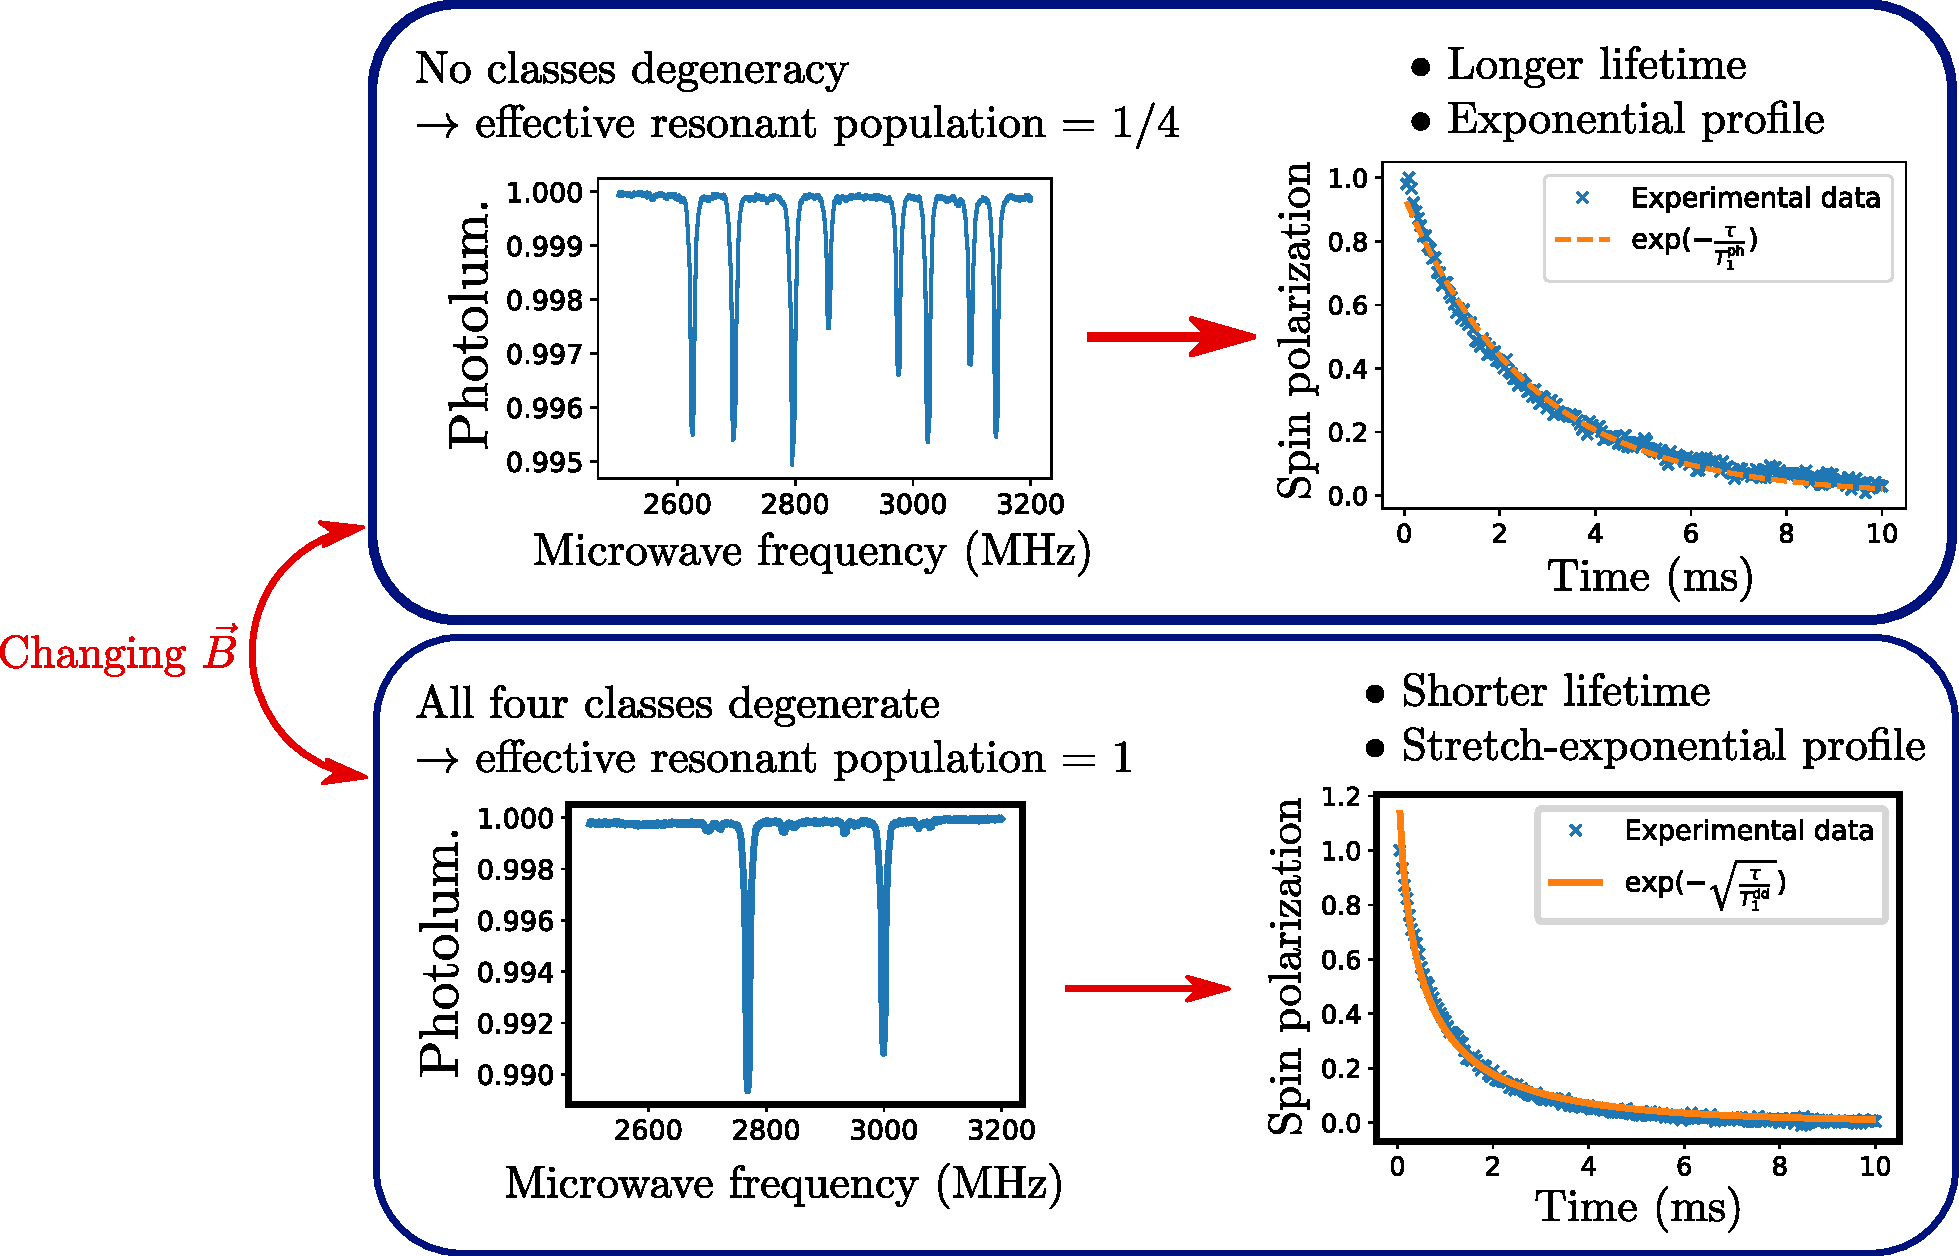
\includegraphics[width=\textwidth,height=0.9\textheight,keepaspectratio]{slide_T1_2}
\end{frame}

\begin{frame}{Optical detection of dark spins}
\centering
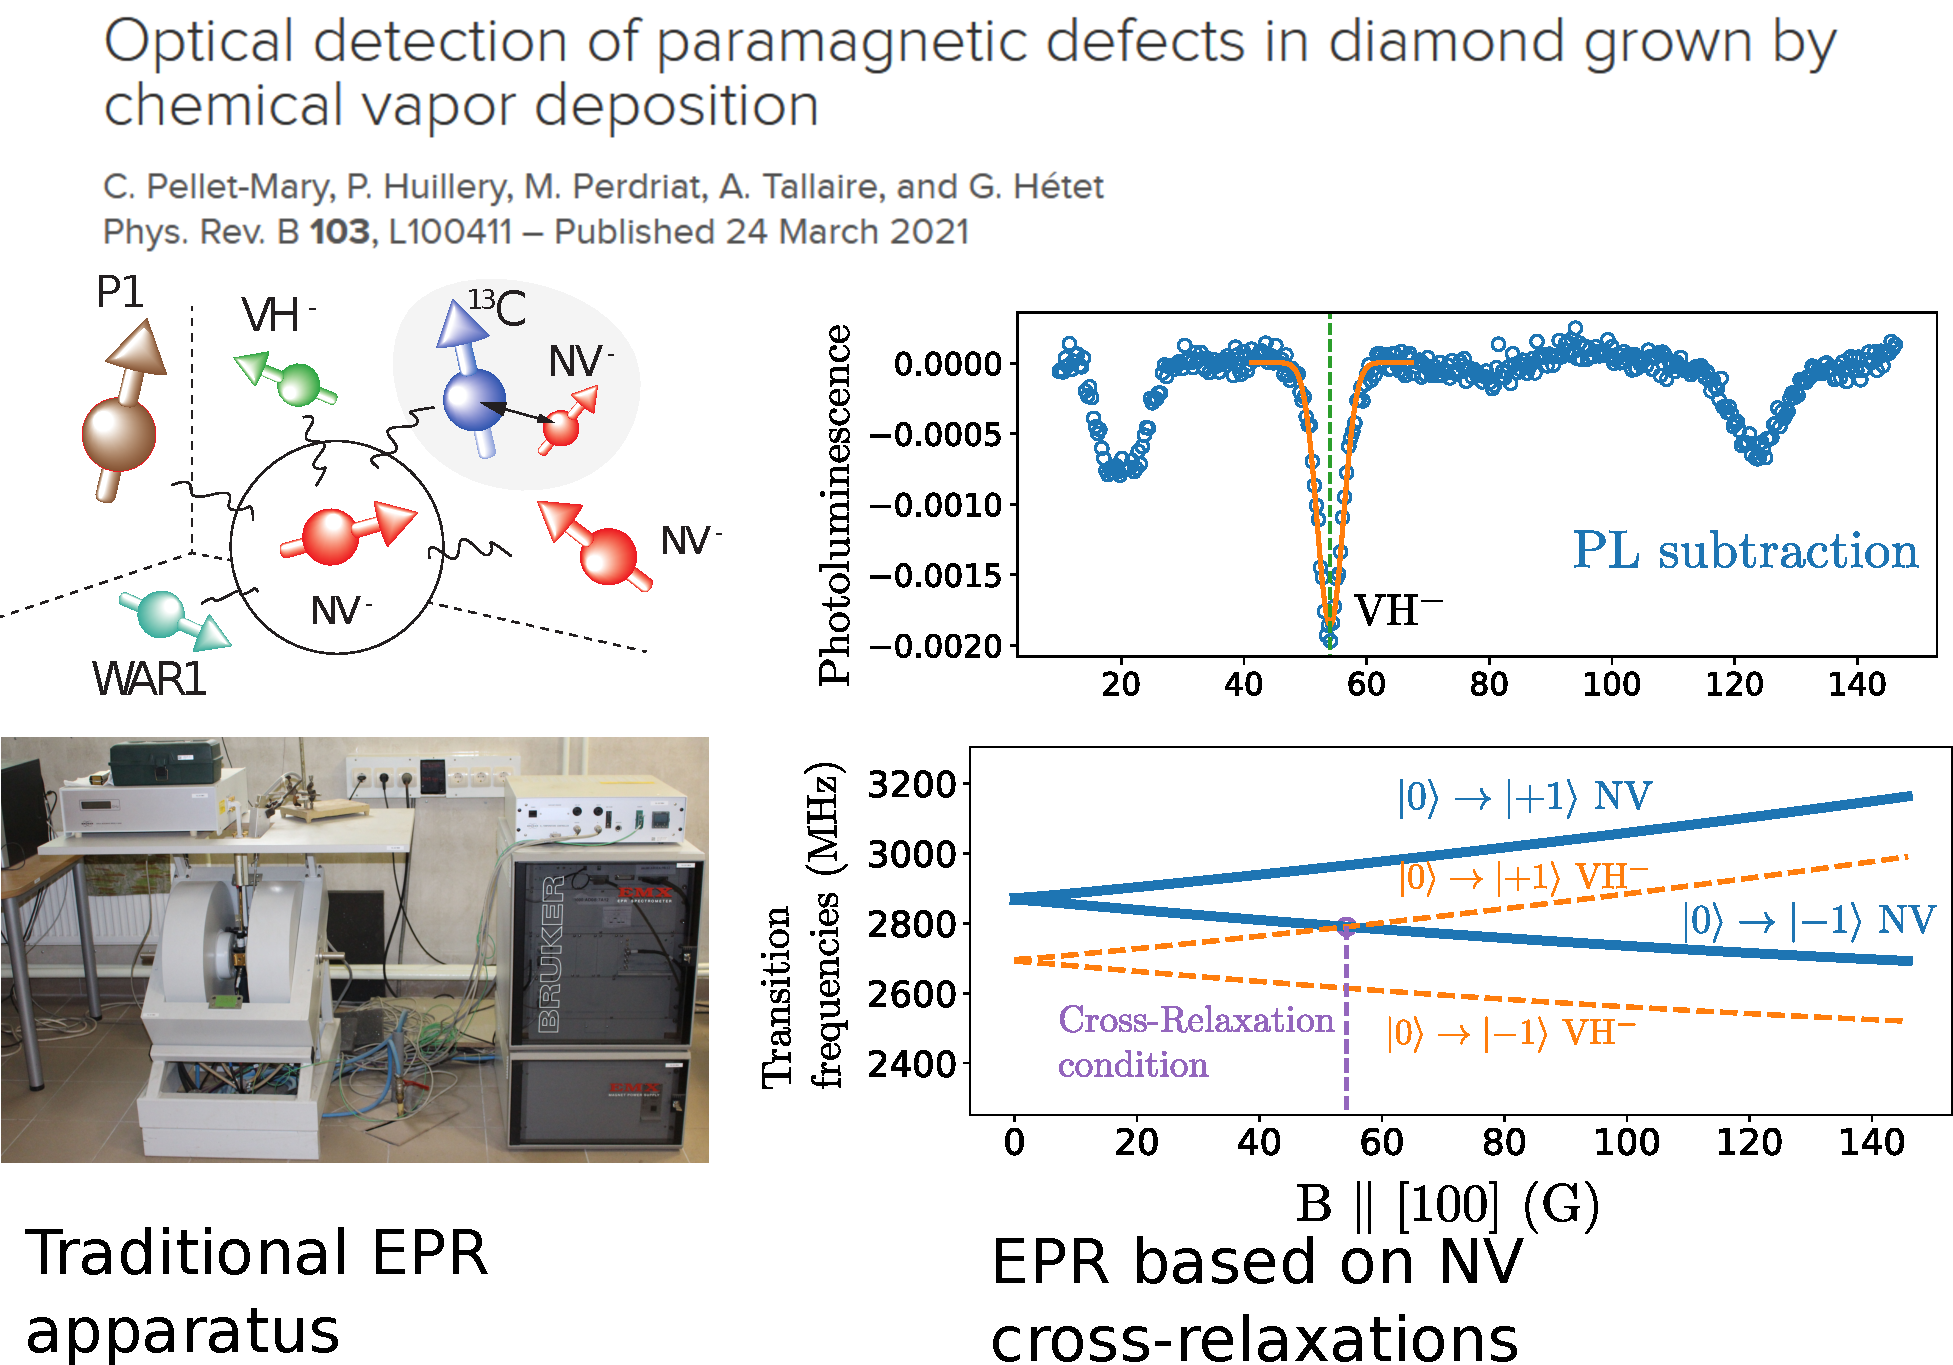
\includegraphics[width=\textwidth,height=0.9\textheight,keepaspectratio]{dark spins}
\end{frame}

\begin{frame}{Mechanical detection of dipole-dipole coupling}
\centering
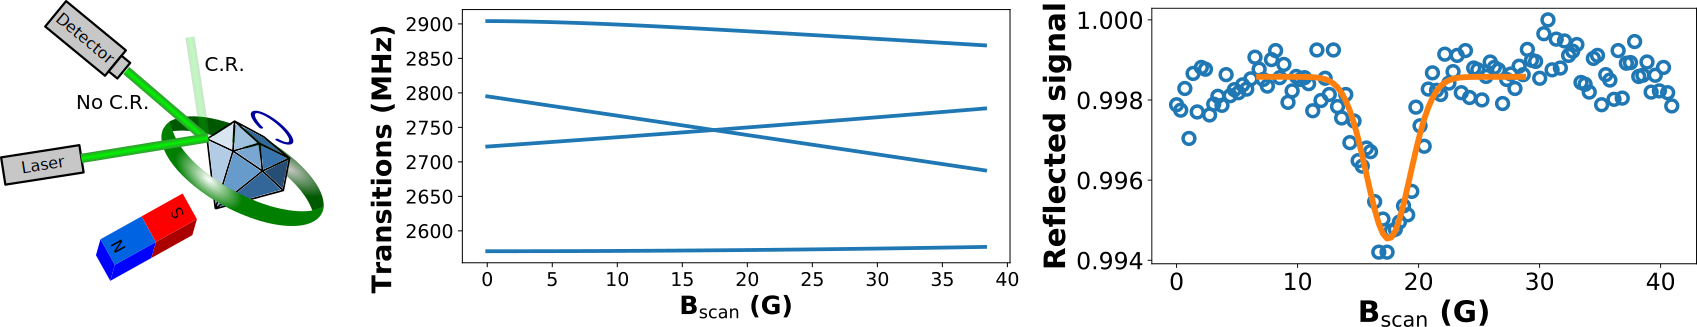
\includegraphics[width=\textwidth,height=0.9\textheight,keepaspectratio]{Cr-meca}
\end{frame}


\begin{frame}{Conclusion}
\textbf{Acknowledgments}  

The team : Gabriel, Maxime, André, the former members : Paul, Louis Tom, the nano-optics group and the technical staff : Christine, Pascal, Arnaud...

\bigskip
\textbf{Take home messages }
\begin{itemize}
\item NV centers are defects in diamond with an optically controllable and readable spin at room temperature
\medskip
\item Many body effects start to manifest with the new NV-rich samples being made
\medskip
\item These effects can be exploited for applications : detection of dark spins, magnetometry, mechanical cooling...
\end{itemize}
\end{frame}
\begin{frame}{Bonus : Magnetometry in zero magnetic field}
\centering
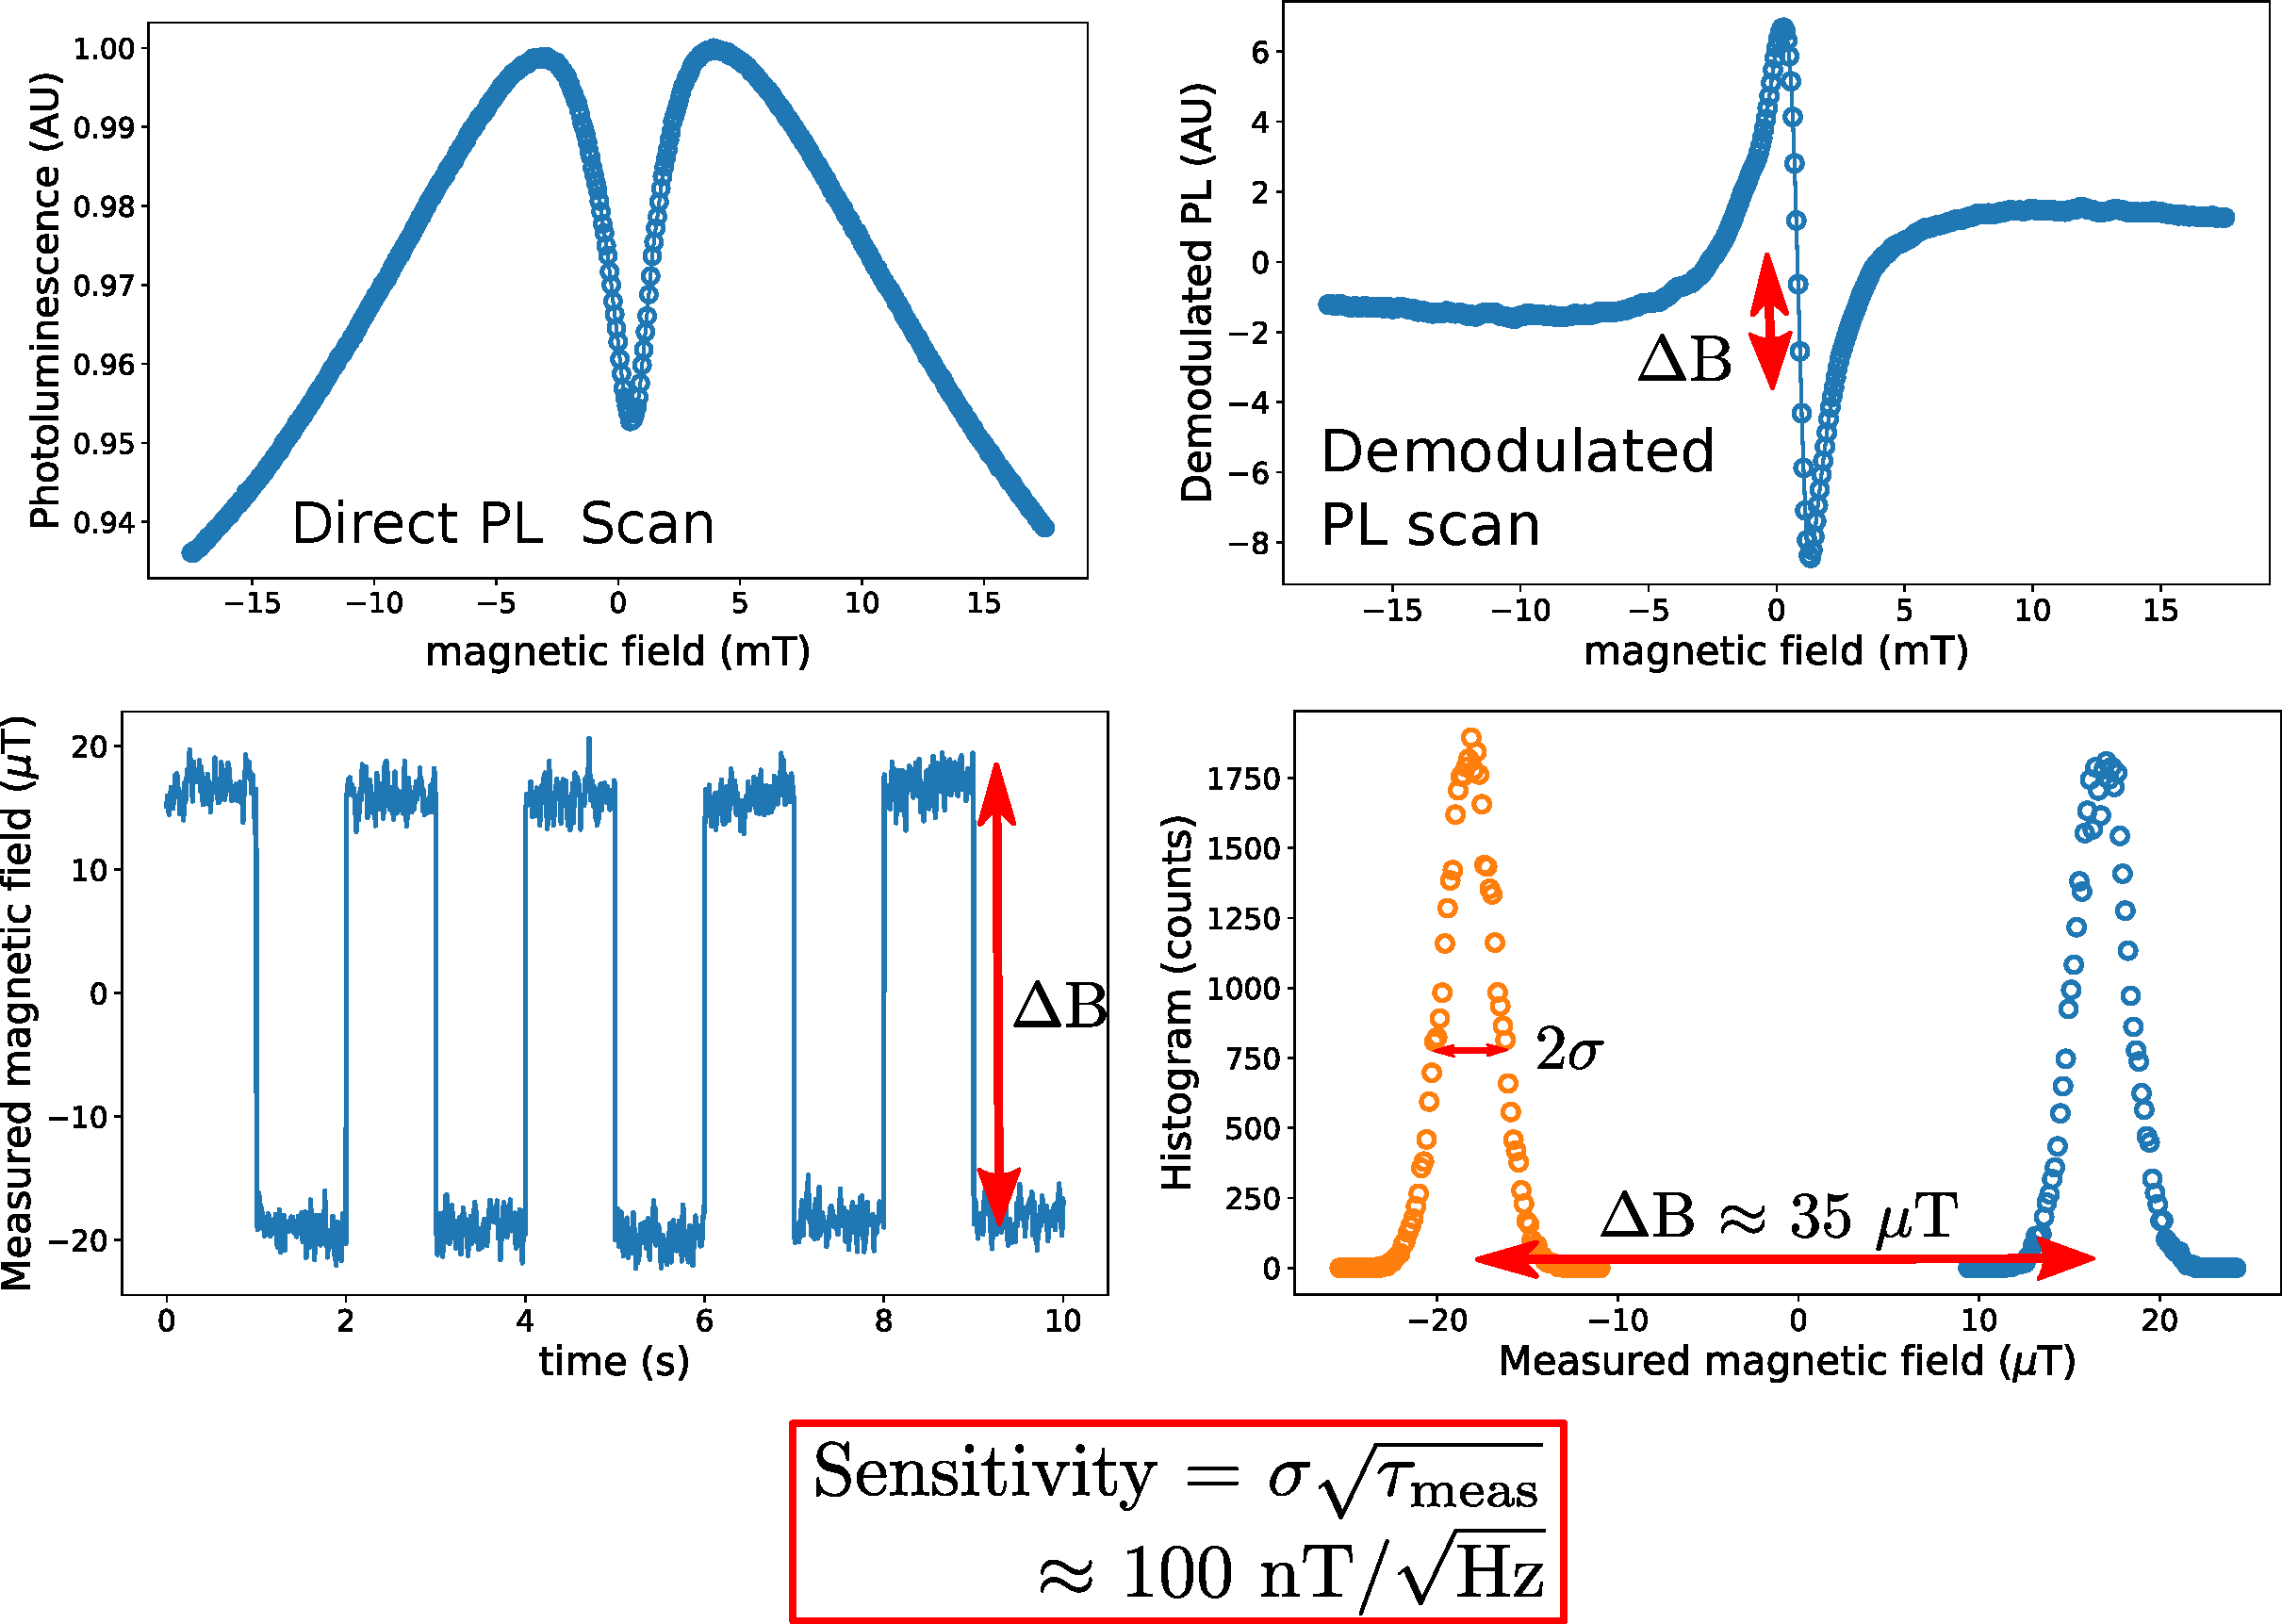
\includegraphics[width=\textwidth,height=0.9\textheight,keepaspectratio]{Slide_magneto}
\end{frame}
\begin{frame}{Optical properties of NV$^-$ centers}
\centering
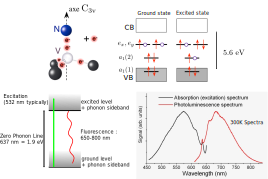
\includegraphics[width=\textwidth,height=0.9\textheight,keepaspectratio]{slide_NV_optical}
\end{frame}
\begin{frame}{NV$^-$ center electronic structure}
\centering
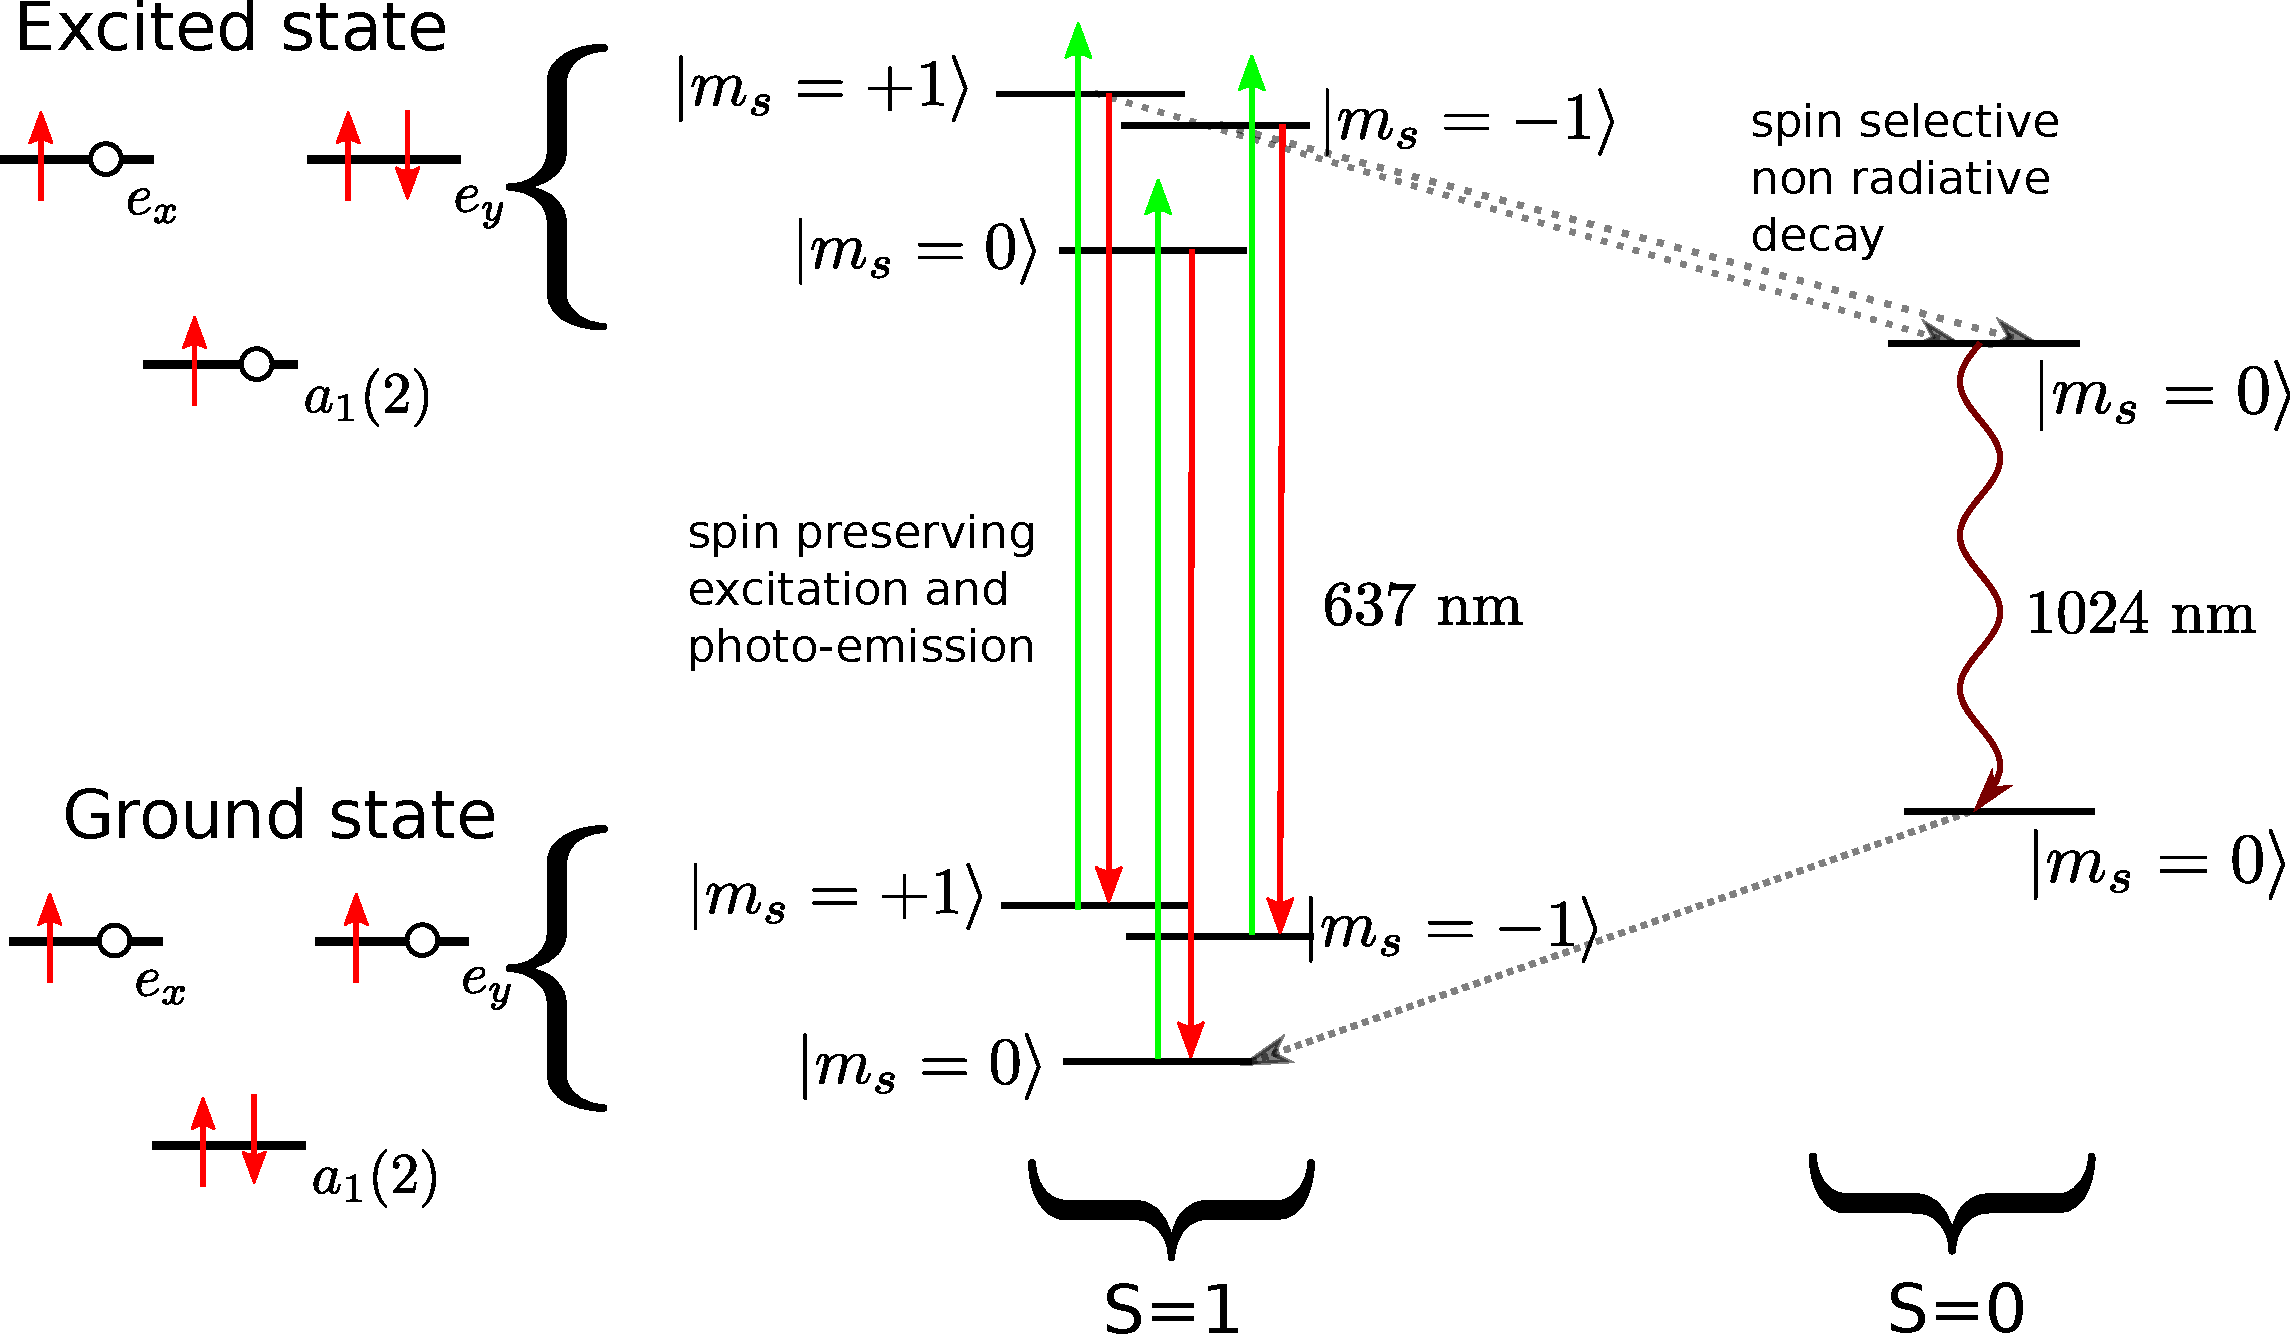
\includegraphics[width=\textwidth,height=0.9\textheight,keepaspectratio]{NV_8_niveaux_3}
\end{frame}
\begin{frame}{NV center spin sub-levels}
\centering
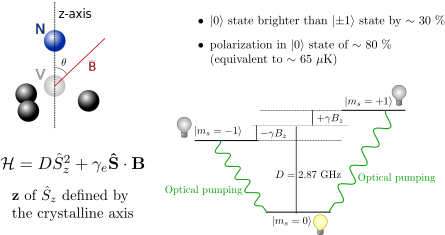
\includegraphics[width=\textwidth,height=0.9\textheight,keepaspectratio]{slide_3_niveaux}
\end{frame}
\end{document}